%--------------------------------------------------------------------
%
%Mustervorlage fuer eine Aufgabe
%
%--------------------------------------------------------------------
%
%Ueberschreiben der automatisch erzeugten Aufgabennummer
%Die folgende Aufgabennummer ergibt sich aus dem Stand des
%Zählers + 1
%\setcounter{chapter}{0}
%
\chapter{}\label{ex:aufg2}
%
%Teilaufgabe 1
%
\section{}\label{sec:aufg2a}
%
In den folgenden Graphiken werden die Signale der Hallsensoren (siehe Abbbildung~\ref{dia:aufg2a_hall}) und die idealisierten Stromverläufe (siehe Abbildung~\ref{dia:aufgabe2a_strom}) dargestellt.
\begin{figure}[htb]
	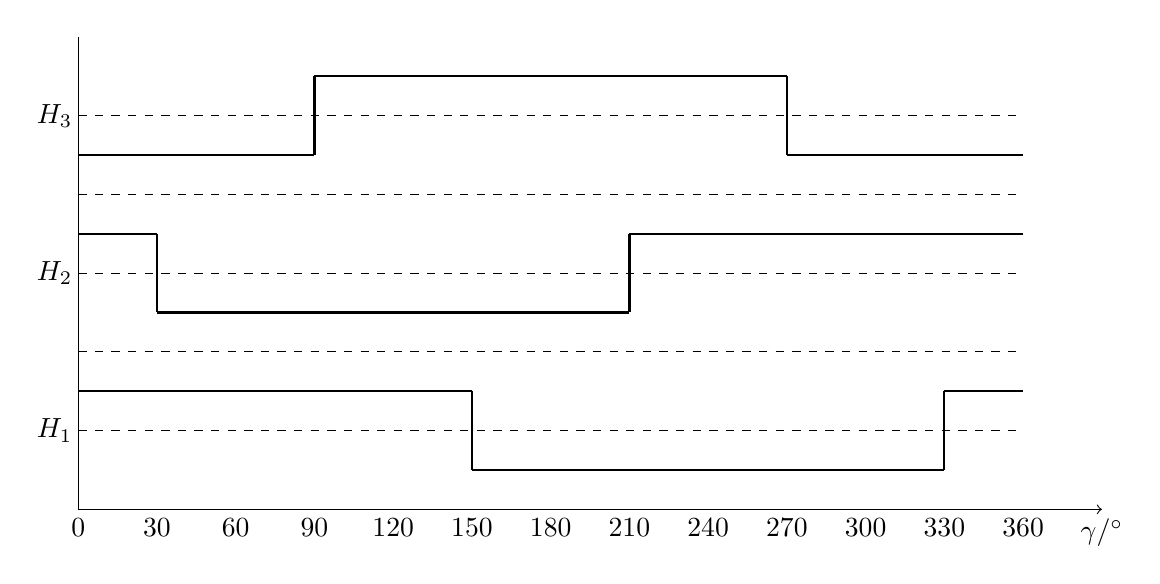
\begin{tikzpicture}
	
	% horizontal axis
	\draw[->] (0,0) -- (13,0) node[anchor=north] {$\gamma/^{\circ}$};
	\draw[dashed] (0, 1) -- (12,1);
	\draw[dashed] (0, 2) -- (12,2);
	\draw[dashed] (0, 3) -- (12,3);
	\draw[dashed] (0, 4) -- (12,4);
	\draw[dashed] (0, 5) -- (12,5);

	% vertical axis
	\draw (0,0) -- (0,6) node[anchor=east] {};

	% labels
	\draw	(0,0) node[anchor=north] {0}
	(1,0) node[anchor=north] {30}
	(2,0) node[anchor=north] {60}
	(3,0) node[anchor=north] {90}	
	(4,0) node[anchor=north] {120}
	(5,0) node[anchor=north] {150}
	(6,0) node[anchor=north] {180}
	(7,0) node[anchor=north] {210}
	(8,0) node[anchor=north] {240}
	(9,0) node[anchor=north] {270}
	(10,0) node[anchor=north] {300}
	(11,0) node[anchor=north] {330}
	(12,0) node[anchor=north] {360};	
	
	\draw (-0.3, 5) node{{$H_3$}};
	\draw (-0.3, 3) node{{$H_2$}};
	\draw (-0.3, 1) node{{$H_1$}};

	%draw H3
	\draw [thick] (0, 4.5) -- (3, 4.5)
	(3, 4.5) -- (3, 5.5)
	(3, 5.5) -- (9, 5.5)
	(9, 5.5) -- (9, 4.5)
	(9, 4.5) -- (12, 4.5);
	
	%draw H2
	\draw [thick] (0, 3.5) -- (1, 3.5)
	(1, 3.5) -- (1, 2.5)
	(1, 2.5) -- (7, 2.5)
	(7, 2.5) -- (7, 3.5)
	(7, 3.5) -- (12, 3.5);
	
	%draw H1
	\draw [thick] (0, 1.5) -- (5, 1.5)
	(5, 1.5) -- (5, 0.5)
	(5, 0.5) -- (11, 0.5)
	(11, 0.5) -- (11, 1.5)
	(11, 1.5) -- (12, 1.5);


	
	\end{tikzpicture}
	\caption{Signale der Hallsensoren - Rechtslauf}
	\label{dia:aufg2a_hall}
\end{figure}

\begin{figure}[htb]
	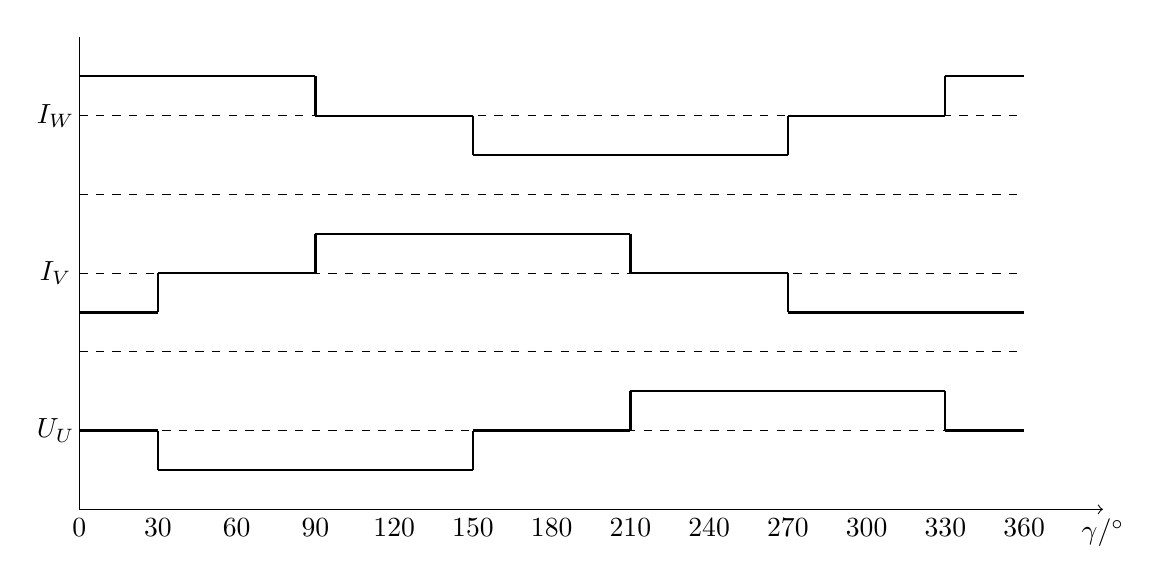
\begin{tikzpicture}
	
	% horizontal axis
	\draw[->] (0,0) -- (13,0) node[anchor=north] {$\gamma/^{\circ}$};
	\draw[dashed] (0, 1) -- (12,1);
	\draw[dashed] (0, 2) -- (12,2);
	\draw[dashed] (0, 3) -- (12,3);
	\draw[dashed] (0, 4) -- (12,4);
	\draw[dashed] (0, 5) -- (12,5);
	
	% vertical axis
	\draw (0,0) -- (0,6) node[anchor=east] {};
	
	% labels
	\draw	(0,0) node[anchor=north] {0}
	(1,0) node[anchor=north] {30}
	(2,0) node[anchor=north] {60}
	(3,0) node[anchor=north] {90}	
	(4,0) node[anchor=north] {120}
	(5,0) node[anchor=north] {150}
	(6,0) node[anchor=north] {180}
	(7,0) node[anchor=north] {210}
	(8,0) node[anchor=north] {240}
	(9,0) node[anchor=north] {270}
	(10,0) node[anchor=north] {300}
	(11,0) node[anchor=north] {330}
	(12,0) node[anchor=north] {360};	
	
	\draw (-0.3, 5) node{{$I_W$}};
	\draw (-0.3, 3) node{{$I_V$}};
	\draw (-0.3, 1) node{{$U_U$}};
	
	%draw Iw
	\draw [thick] 
	(0, 5.5)  --  (3, 5.5)
	(3, 5.5)  --  (3, 5.0)
	(3, 5.0)  --  (5, 5.0)
	(5, 5.0)  --  (5, 4.5)
	(5, 4.5)  --  (9, 4.5)
	(9, 4.5)  --  (9, 5.0)
	(9, 5.0)  -- (11, 5.0)
	(11, 5.0) -- (11, 5.5)
	(11, 5.5) -- (12, 5.5);
	
	%draw Iv
	\draw [thick] 
	(0, 2.5)  --  (1, 2.5)
	(1, 2.5)  --  (1, 3.0)
	(1, 3.0)  --  (3, 3.0)
	(3, 3.0)  --  (3, 3.5)
	(3, 3.5)  --  (7, 3.5)
	(7, 3.5)  --  (7, 3.0)
	(7, 3.0)  --  (9, 3.0)
	(9, 3.0)  --  (9, 2.5)
	(9, 2.5)  -- (12, 2.5);
	
	%draw Iu
	\draw [thick] 
	(0, 1.0)  --  (1, 1.0)
	(1, 1.0)  --  (1, 0.5)
	(1, 0.5)  --  (5, 0.5)
	(5, 0.5)  --  (5, 1.0)
	(5, 1.0)  --  (7, 1.0)
	(7, 1.0)  --  (7, 1.5)
	(7, 1.5)  -- (11, 1.5)
	(11, 1.5) -- (11, 1.0)
	(11, 1.0) -- (12, 1.0);
	
	\end{tikzpicture}
	\caption{Idealisierte Stromverl\"aufe}
	\label{dia:aufgabe2a_strom}
\end{figure}
\newpage
%
%--------------------------------------------------------------------
%
%Teilaufgabe 2
%
\section{}\label{sec:aufg2b}
%
Im folgenden Diagramm (siehe Abbildung~\ref{dia:2b_ansteuersig}) werden die Ansteuersignale der sechs Transistoren für den Rechtslauf dargestellt. Der Einfachheit halber werden für $W$,$V$ und $U$ je Highside leitend als $1$, Lowside leitend als $-1$ und gesperrt als $0$ bezeichnet. Somit gleichen die Ansteuersignale dem idealisierten Stromverlauf aus dem Skript elektische Antriebe S.102, Abbildung 8.3.
\begin{figure}[htb]
	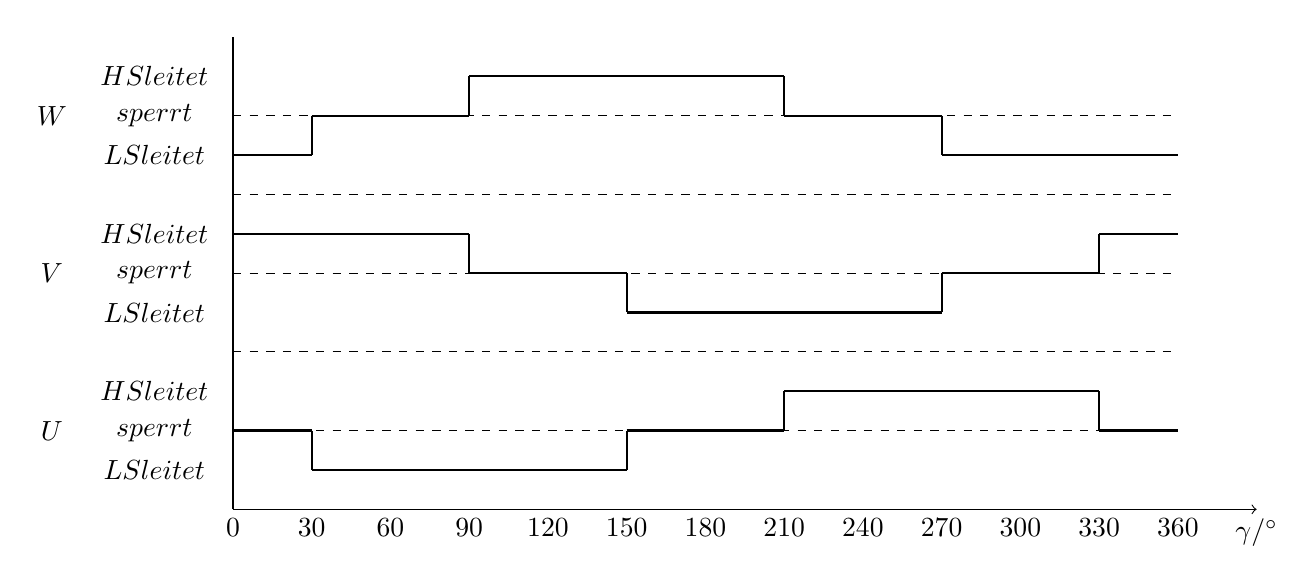
\begin{tikzpicture}
	
		% horizontal axis
		\draw[->] (0,0) -- (13,0) node[anchor=north] {$\gamma/^{\circ}$};
		\draw[dashed] (0, 1) -- (12,1);
		\draw[dashed] (0, 2) -- (12,2);
		\draw[dashed] (0, 3) -- (12,3);
		\draw[dashed] (0, 4) -- (12,4);
		\draw[dashed] (0, 5) -- (12,5);
		
		% vertical axis
		\draw (0,0) -- (0,6) node[anchor=east] {};
		
		% labels
		\draw	(0,0) node[anchor=north] {0}
		(1,0) node[anchor=north] {30}
		(2,0) node[anchor=north] {60}
		(3,0) node[anchor=north] {90}	
		(4,0) node[anchor=north] {120}
		(5,0) node[anchor=north] {150}
		(6,0) node[anchor=north] {180}
		(7,0) node[anchor=north] {210}
		(8,0) node[anchor=north] {240}
		(9,0) node[anchor=north] {270}
		(10,0) node[anchor=north] {300}
		(11,0) node[anchor=north] {330}
		(12,0) node[anchor=north] {360};	
		
		\draw (-2.3, 5) node{{$W$}};
			\draw (-1, 5.5) node{{$HS leitet$}};
			\draw (-1, 5) node{{$sperrt$}};
			\draw (-1, 4.5) node{{$LS leitet$}};
		\draw (-2.3, 3) node{{$V$}};
			\draw (-1, 3.5) node{{$HS leitet$}};
			\draw (-1, 3) node{{$sperrt$}};
			\draw (-1, 2.5) node{{$LS leitet$}};
		\draw (-2.3, 1) node{{$U$}};
			\draw (-1, 1.5) node{{$HS leitet$}};
			\draw (-1, 1) node{{$sperrt$}};
			\draw (-1, 0.5) node{{$LS leitet$}};
		
		%draw W
		\draw [thick] 
		(0, 4.5)  --  (1, 4.5)
		(1, 4.5)  --  (1, 5.0)
	 	(1, 5.0)  --  (3, 5.0)
		(3, 5.0)  --  (3, 5.5)
		(3, 5.5)  --  (7, 5.5)
		(7, 5.5)  --  (7, 5.0)
		(7, 5.0)  --  (9, 5.0)
		(9, 5.0)  --  (9, 4.5)
		(9, 4.5)  -- (12, 4.5);
		
		%draw V
		\draw [thick] 
		(0, 3.5)  --  (3, 3.5)
		(3, 3.5)  --  (3, 3.0)
		(3, 3.0)  --  (5, 3.0)
		(5, 3.0)  --  (5, 2.5)
		(5, 2.5)  --  (9, 2.5)
		(9, 2.5)  --  (9, 3.0)
		(9, 3.0)  -- (11, 3.0)
		(11, 3.0) -- (11, 3.5)
		(11, 3.5) -- (12, 3.5);
		
		%draw U
		\draw [thick] 
		(0, 1.0)  --  (1, 1.0)
		(1, 1.0)  --  (1, 0.5)
		(1, 0.5)  --  (5, 0.5)
		(5, 0.5)  --  (5, 1.0)
		(5, 1.0)  --  (7, 1.0)
		(7, 1.0)  --  (7, 1.5)
		(7, 1.5)  -- (11, 1.5)
		(11, 1.5) -- (11, 1.0)
		(11, 1.0) -- (12, 1.0);
	
	\end{tikzpicture}
	\caption{Ansteuersignale der 6 Transistoren - Rechtslauf}
	\label{dia:2b_ansteuersig}
\end{figure}
%
\section{}\label{sec:aufg2c}
%
Die Ansteuerung der Transistoren entspricht wie in \ref{sec:aufg2b}) erwähnt  dem idealisierten Stromverlauf.
\begin{figure}[htb]
	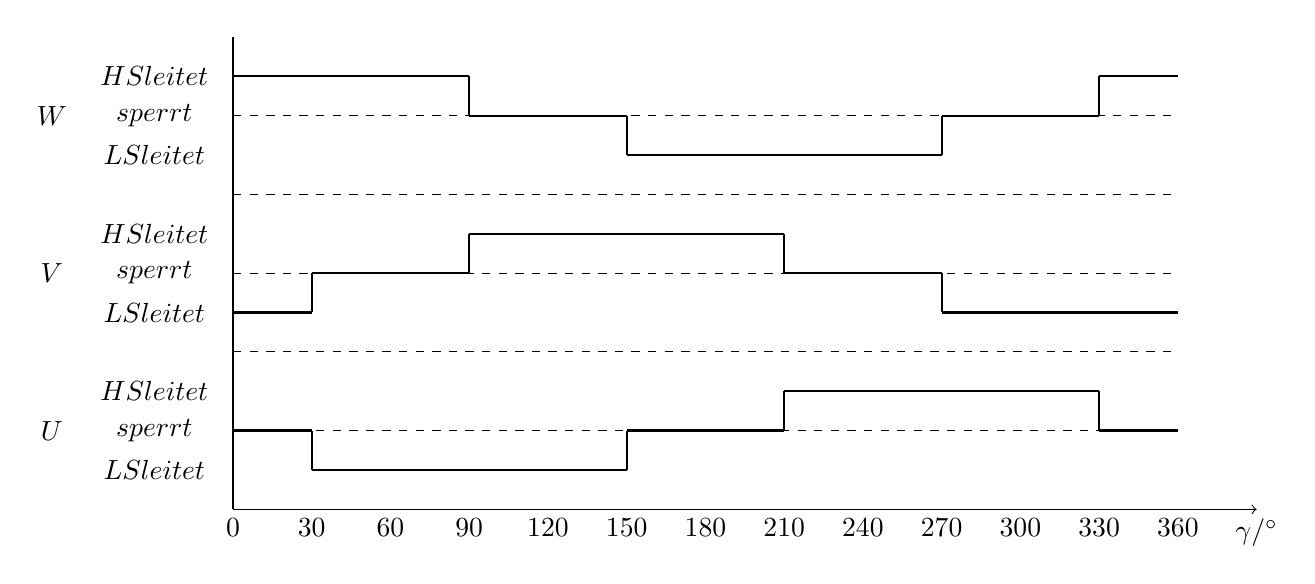
\begin{tikzpicture}
	
		% horizontal axis
		\draw[->] (0,0) -- (13,0) node[anchor=north] {$\gamma/^{\circ}$};
		\draw[dashed] (0, 1) -- (12,1);
		\draw[dashed] (0, 2) -- (12,2);
		\draw[dashed] (0, 3) -- (12,3);
		\draw[dashed] (0, 4) -- (12,4);
		\draw[dashed] (0, 5) -- (12,5);
		
		% vertical axis
		\draw (0,0) -- (0,6) node[anchor=east] {};
		
		% labels
		\draw	(0,0) node[anchor=north] {0}
		(1,0) node[anchor=north] {30}
		(2,0) node[anchor=north] {60}
		(3,0) node[anchor=north] {90}	
		(4,0) node[anchor=north] {120}
		(5,0) node[anchor=north] {150}
		(6,0) node[anchor=north] {180}
		(7,0) node[anchor=north] {210}
		(8,0) node[anchor=north] {240}
		(9,0) node[anchor=north] {270}
		(10,0) node[anchor=north] {300}
		(11,0) node[anchor=north] {330}
		(12,0) node[anchor=north] {360};	
		
		\draw (-2.3, 5) node{{$W$}};
			\draw (-1, 5.5) node{{$HS leitet$}};
			\draw (-1, 5) node{{$sperrt$}};
			\draw (-1, 4.5) node{{$LS leitet$}};
		\draw (-2.3, 3) node{{$V$}};
			\draw (-1, 3.5) node{{$HS leitet$}};
			\draw (-1, 3) node{{$sperrt$}};
			\draw (-1, 2.5) node{{$LS leitet$}};
		\draw (-2.3, 1) node{{$U$}};
			\draw (-1, 1.5) node{{$HS leitet$}};
			\draw (-1, 1) node{{$sperrt$}};
			\draw (-1, 0.5) node{{$LS leitet$}};
		
		%draw W
		\draw [thick] 
		(0, 5.5)  --  (3, 5.5)
		(3, 5.5)  --  (3, 5.0)
		(3, 5.0)  --  (5, 5.0)
		(5, 5.0)  --  (5, 4.5)
		(5, 4.5)  --  (9, 4.5)
		(9, 4.5)  --  (9, 5.0)
		(9, 5.0)  -- (11, 5.0)
		(11, 5.0) -- (11, 5.5)
		(11, 5.5) -- (12, 5.5);
		
		%draw V
		\draw [thick] 
		(0, 2.5)  --  (1, 2.5)
		(1, 2.5)  --  (1, 3.0)
		(1, 3.0)  --  (3, 3.0)
		(3, 3.0)  --  (3, 3.5)
		(3, 3.5)  --  (7, 3.5)
		(7, 3.5)  --  (7, 3.0)
		(7, 3.0)  --  (9, 3.0)
		(9, 3.0)  --  (9, 2.5)
		(9, 2.5)  -- (12, 2.5);
		
		%draw U
		\draw [thick] 
		(0, 1.0)  --  (1, 1.0)
		(1, 1.0)  --  (1, 0.5)
		(1, 0.5)  --  (5, 0.5)
		(5, 0.5)  --  (5, 1.0)
		(5, 1.0)  --  (7, 1.0)
		(7, 1.0)  --  (7, 1.5)
		(7, 1.5)  -- (11, 1.5)
		(11, 1.5) -- (11, 1.0)
		(11, 1.0) -- (12, 1.0);
	
	\end{tikzpicture}
	\caption{Ansteuersignale der 6 Transistoren - Linkslauf}
	\label{dia:2c_ansteuersig}
\end{figure}
%
\newpage
\section{}\label{sec:aufg2d}
%
Wir nutzen die Formel 5.9 aus dem Vorlesungsskript S.41.
\begin{equation}
	U_a = R_a I_a(t) + L_a \frac{dI_a(t)}{dt} + U_I
	\label{for:formel1}
\end{equation}

Mit $U_I = 0$ gilt:
\begin{equation}
    L_a\frac{dI_a(t)}{dt} + R_a I_a(t) = U_a
	\label{for:formel2}
\end{equation}

Umgeformt ergibt sich:
\begin{equation}
	\tau\frac{dI_a(t)}{dt} + I_a(t) = \frac{U_a}{R_a}
\end{equation}

Wobei für die Zeitkonstante $\tau = \frac{L_a}{R_a}$ gilt.\\
Die Lösung dieser Differentialgleichung lautet:
\begin{equation}
	I_a(t) = \frac{U_a}{R_a}(1-e^-\frac{t-1ms}{\tau})
\end{equation}
Für $R_a = 0.8\Omega$ und $L_a = 1.1$mH und einem Spannungsverlauf, wie im Skript (siehe S.105 Abbildung~8.7) dargestellt, ergibt es im Strang U einen Ankerstrom der folgendermaßen verläuft (siehe Abbildung~\ref{fig:ankerstrom}):
\begin{figure}[htb]
	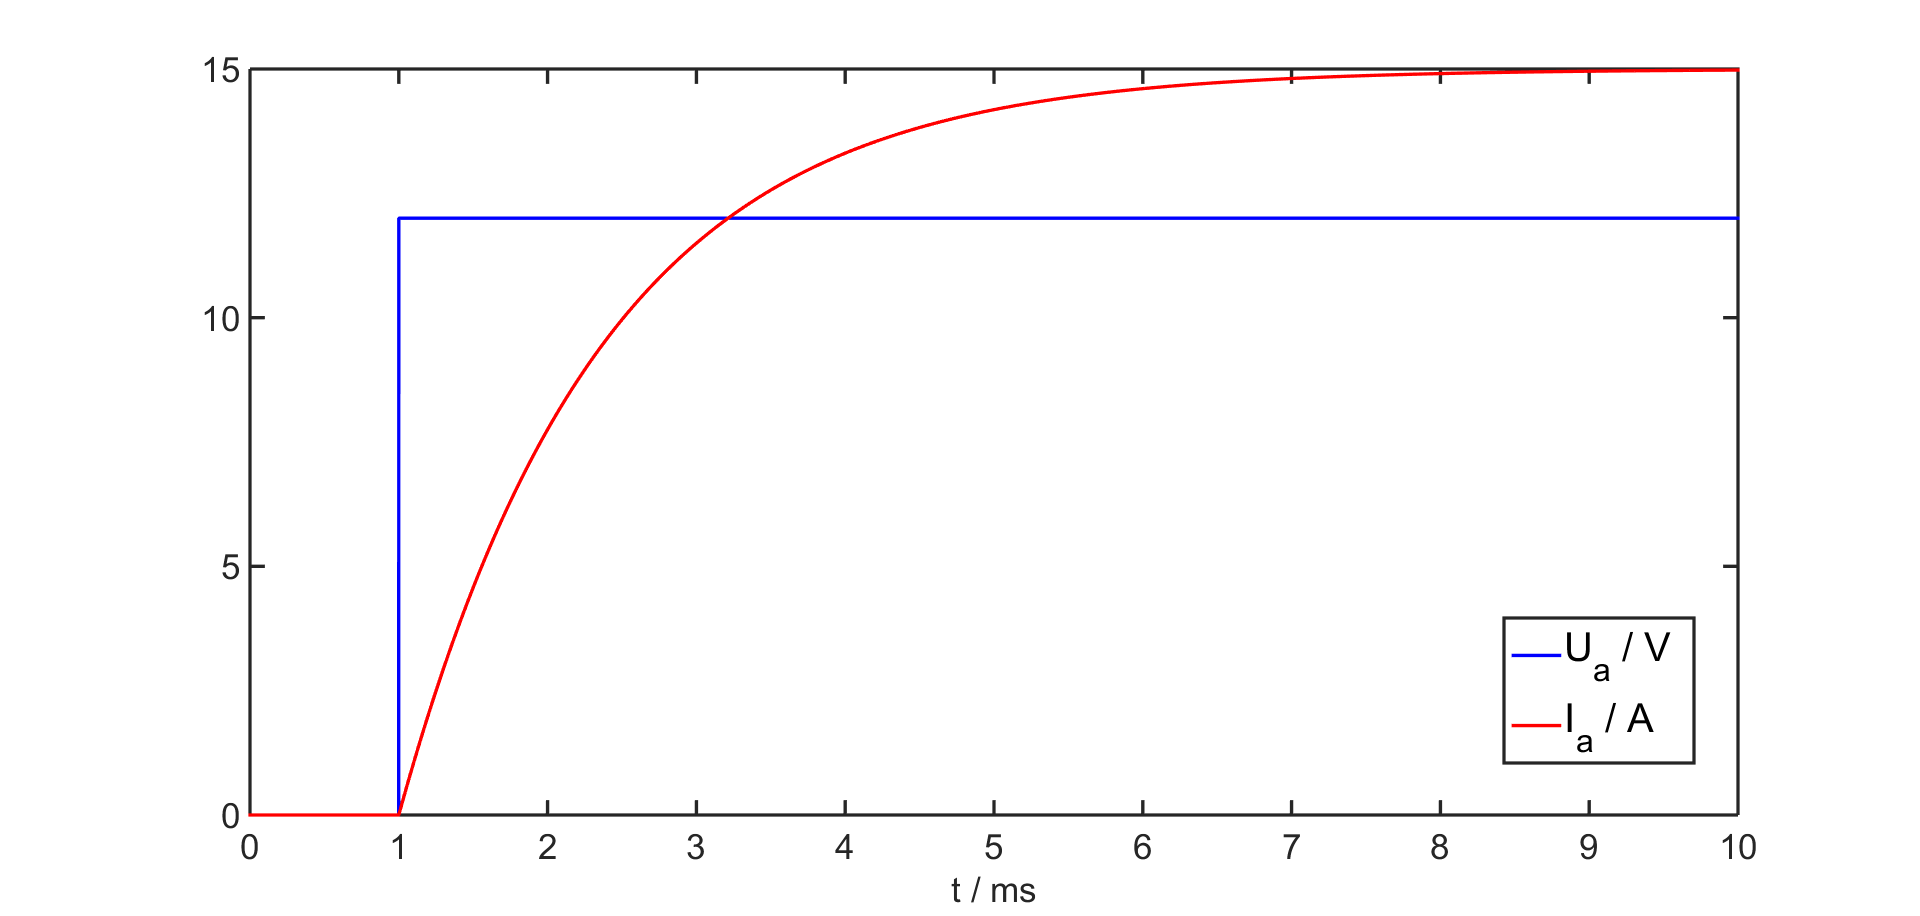
\includegraphics[width=\textwidth]{./Bilder/Ankerstrom_Aufgabe2d}
	\caption{Verlauf des Ankerstroms}
	\label{fig:ankerstrom}
\end{figure}




%\begin{tikzpicture}

\begin{axis}[xmax = 10, ymax = 15, samples=100]
\addplot[blue, ultra thick] (x,x*x)
\end{axis}

\end{tikzpicture}

%Alle bisherigen Bilder einfügen und einen Seitenumbruch erzwingen
\clearpage
